\documentclass[preprint]{llncs}
\usepackage{etex}

%\usepackage{color}

%\usepackage{amsmath}
%\usepackage{stmaryrd}
\usepackage{graphicx}
\usepackage{amssymb}
\usepackage{url}
%\usepackage{bbm}
%\usepackage{pgf}
%\usepackage{multirow}
\usepackage{listings}
\usepackage{verbatim}
%\usepackage{graphicx}
%\usepackage{wrapfig}
\usepackage{xspace}
\usepackage{ql}

\usepackage[T1]{fontenc}
\usepackage[scaled=0.85]{beramono}
%\usepackage{dirtree}

\lstset{ %
language=Java,                % choose the language of the code
columns=flexible,
lineskip=-1pt,
basicstyle=\ttfamily\small,       % the size of the fonts that are used for the code
numbers=none,                   % where to put the line-numbers
numberstyle=\ttfamily\tiny,      % the size of the fonts that are used for the line-numbers
stepnumber=1,                   % the step between two line-numbers. If it's 1 each line will be numbered
numbersep=5pt,                  % how far the line-numbers are from the code
backgroundcolor=\color{white},  % choose the background color. You must add \usepackage{color}
showspaces=false,               % show spaces adding particular underscores
showstringspaces=false,         % underline spaces within strings
showtabs=false,                 % show tabs within strings adding particular underscores
morekeywords={var},
%  frame=single,                   % adds a frame around the code
tabsize=2,                  % sets default tabsize to 2 spaces
captionpos=none,                   % sets the caption-position to bottom
breaklines=true,                % sets automatic line breaking
breakatwhitespace=false,        % sets if automatic breaks should only happen at whitespace
title=\lstname,                 % show the filename of files included with \lstinputlisting; also try caption instead of title
escapeinside={(*}{*)},          % if you want to add a comment within your code
keywordstyle=\ttfamily\bfseries,
% commentstyle=\color{Gray},
% stringstyle=\color{Green}
}

\pagestyle{plain}


\newcommand{\authornote}[3]{{\color{#2} {\sc #1}: #3}}
\newcommand\jason[1]{\authornote{jason}{green}{#1}}
\newcommand\haoyuan[1]{\authornote{haoyuan}{red}{#1}}
\newcommand\bruno[1]{\authornote{bruno}{red}{#1}}
\newcommand\tijs[1]{\authornote{tijs}{blue}{#1}}

\newcommand\name{{\bf Shy}\xspace}
\newcommand\Name{{\bf Shy}\xspace}

\newcommand{\hl}[1]{\textcolor{red}{#1}}

\newcommand\sem[1]{\llbracket #1 \rrbracket_r}
\newcommand\sems[1]{\llbracket #1 \rrbracket_s}
\newcommand\tsem[1]{\llbracket #1 \rrbracket}
\newcommand{\rbm}[1]{\raisebox{-2.0ex}[0.5ex]{#1}}
\newcommand\nat[0]{\mathbb{N}}
\newcommand\unit[0]{\mathbbm{1}}

\author{Hoayuan Zhang$^{\textrm{1}}$ Jason Chu$^{\textrm{2}}$ }
\institute{$^{\textrm{1}}$The University of Hong Kong\\
\email{author1@cs.hku.hk}\\
$^{\textrm{2}}$ The University of Hong Kong\\
\email{author2@cs.hku.hk}}
\authorrunning{Haoyuan Zhang et al.} % abbreviated author list (for running head)


%%%%%%%%%%%%%%%%%%%%%%%%%%%%%%%%%%%%%%%%%%%%%%%%%%%%%%%%%%%%%%%%%%%%%%%%%%%%%%%%
\begin{document}

%%\conferenceinfo{POPL'10} {}
%%\CopyrightYear{2010}


\title{Scrap your Boilerplate with Object Algebras}

\maketitle

\begin{abstract}

Traversing complex data structures typically requires large amounts of
tedious boilerplate code. For many operations most of the code simply
walks the structure, and only a small portion of the code implements
the functionality that motivated the traversal in the first place.
This paper present a type-safe Java framework called \name that
removes much of this boilerplate code. In \name \emph{object algebras}
are used to describe complex \emph{extensible} data structures. Using
Java annotations generic boilerplate code is generated for various
types of traversals, including queries and transformations.  Thus,
using \Name, programmers can inherit the generic traversal code to
focus only on writing the interesting parts of the
traversals. Consequently, the amount of code that programmers need to
write is significantly smaller. Moreover, traversals using the \name framework
are also much more \emph{structure shy}, becoming more adaptive
to future changes or extensions to the data structure.
%An additional benefit of \name is that traversal code can be easily
%reused by extensions of the
To prove the effectiveness of the approach, we employeed \name
on the implementation of a domain-specific questionaire
language. Our results show that for a large number of traversals
there was a significant reduction in the amount of user-defined code.
%\bruno{Say something more about extensibility and type-safety!}

\begin{comment}

Static types are useful to distinguish between different kinds
of nodes in a structure and to prevent misuses. The
distinction between different types of nodes also means that code for
dealing with each type of node is needed. However, in large structures,
such as the Abstract Syntax Tree (AST) of a programming language,
the amount of required code can be a problem. For some operations,
which traverse large structures, most of the code amounts to recursively
delegating the traversal to the child nodes. Only for some nodes
of the structure the code needs to do something different. Still
the programmer needs to diligently and tediously write the error-prone
traversal code for all nodes.

In this paper we present a framework

This approach works well for many operations,
which need different (and non-trivial) code for each different type
of node

%Unfortunately, for some operations the interesting

%%In large structures,
%%such as the Abstract Syntax Tree (AST) of a programming language,
%%the code required to traverse the whole structure is proportionaly large.


The problem is particularly prominent
in statically typed languages, where the typing discipline
enforces strict distinctions between different cases

Operations that traverse complex structures often require large and
tedious amounts of boilerplate code. In those operations there are
typically a few

A pervasive problem in programming occurs when large tree tr

\end{comment}

\end{abstract}

%===============================================================================

\section{Introduction}

Various language processing tools or libraries for programming
languages, domain-specific languages, mark-up languages like HTML, or
data-interchange languages like XML or JSON require complex
\emph{Abstract Syntax Tree} (AST) structures. In those applications
ASTs are the key data structure needed to model the various constructs
of these languages. Such ASTs have various different types of nodes,
which can range from a few dozen to several hundred kinds of nodes
(for example in the ASTs of languages like Java or Cobol).

Static types are helpful to deal with such complex ASTs.  Static
types formalize the distinction between different kinds of
nodes. Furthermore the distinctions are helpful to ensure that
traversals over these ASTs have an appropriate piece of code
that deals with each different type of node. This can prevent a large
class of run-time errors that would not otherwise be detected.

%For example static types prevent errors that would arize from
%applying the code intended for a certain kind of node to another kind
%of node. Static types can also ensure that all nodes are dealt with by
%an appropriate piece of code.

Unfortunately, when traversing such ASTs, the number of nodes and the
enforced type distinctions between nodes can lead to so-called
\emph{boilerplate code}~\cite{ralf03syb}: code that is similar for most types of nodes and which
essentially just walks the structure. Operations where the ``interesting'' code is limited to only a small portion of nodes are called \emph{structure shy}~\cite{DemeterBook}.
A typical example is computing the free
variables of an expression in some programming language. In this
case, the interesting code occurs in the nodes representing the
binding and variable constructs. In all other cases, the code would just deal with
walking the structure. In ASTs with dozens or hundreds of
kinds of nodes, having to explicitly write code for each kind of node is both tedious and error-prone.
%In summary, structure shy operations
%suffer from the static typing discipline, because the type
%distinctions between different kinds of nodes leads to significant
%boilerplate code.

The boilerplate problem in implementing traversals has received
considerable attention in the past. For example, both \emph{Adaptive
  Object-Oriented Programming} (AOOP)~\cite{DemeterBook} and
\emph{Strategic Programming}~\cite{borovansky1996elan,visser1998core}
are aimed partly at solving this problem. Most approaches to AOOP and
strategic programming use some meta-programming techniques, such as
code generation or reflection. The use of meta-programming offers
programmers an easy way to avoid having to write boilerplate code.
This has important benefits: users have to write much less code; and 
the code becomes much more adaptive to changes.
%Firstly the user has to write much less
%code, also removing the possibility of errors in the code walking the
%structure. Secondly the code becomes much more adaptive to changes: if
%a change to the traversed data type only affects the generated
%boilerplate code, the user-defined code can remain unchanged. 
However such meta-programming based approaches usually come at the cost of
other desirable properties, such as type-safety, extensibility or
separate compilation. The functional programming community has also
studied the problem before. For instance, the popular ``\emph{Scrap your
boilerplate}''~\cite{ralf03syb} approach supports type-safety and
separate compilation. However most of the techniques used in
functional languages cannot be easily ported to mainstream OO
languages like Java, and are limited in terms of extensibility.


%Object
%algebras are a recently introduced technique, which has been shown to
%have significant advantages for software extensibility. 

This paper presents a Java framework called \name that allows users to
define type-safe and extensible structure-shy operations. \name
uses \emph{Object Algebras}~\cite{bruno12oa} to describe ASTs, and to
write operations over ASTs in a style similar to writing folds in
functional programming. However unlike standard folds in
functional programming, Object Algebras are
\emph{extensible}: when new kinds of nodes are introduced in the data type, the operations can be extended as well, without changing exsting code. 

In \name Object Algebra interfaces are combined
with Java annotations to generate generic traversal code automatically. The
generated code accounts for four different types of traversals:
\emph{queries}; \emph{transformations}; \emph{generalized queries};
and \emph{contextual transformations}.  Each of these four types of
traversals is implemented as an Object Algebra. Programmers who want
to implement structure-shy traversals can then inherit from one of these
four object algebras, and override only the cases that deal with 
the interesting parts of the traversal. Consequently
traversals written in \name are:

\begin{itemize*}

\item {\bf Small in size:} With \name the amount of code that
  programmers need to write a structure-shy traversal is significantly smaller.
  Often traversals in \name are implementable in just a few lines
  of code, even for complex ASTs with hundreds of different types of
  nodes.

\item {\bf Adaptive and structure shy:}  Traversals writen with \name can omit
  boilerplate code, making traversals more adaptive to
  future changes or extensions to the data type.

\item {\bf Type-safe:} \name traversals are directly written in Java
  and the Java type-system ensures type-safety. No run-time casts are
  needed for generic traversal code or for user-defined traversal
  code. 

\item {\bf Extensible with separate compilation:} Traversals inherit type-safe
  extensibility from object algebras. Both traversals and the AST structures
  are extensible. Thus it is possible to
  reuse traversal code for ASTs extended with additional
  node types. Furthermore \name traversals support separate compilation.

\item {\bf Implemented in plain Java:} \name traversals do not require
  a new tool or language. The approach is library based and only uses
  Java annotations.

%\item {\bf Performant:} Traversals written with \name have performance that
%is comparable to naive hand-written OO code.

\end{itemize*}

To prove the effectiveness of the approach, we have applied \name in
the implementation of QL, a domain-specific language (DSL) for defining questionnaires that has been used before as a benchmark language~\cite{gouseti14extensible,erdweg2013state}.  Our results (see details in
Section~\ref{sec:case_study}) show that for a large number of traversals there was a
significant reduction in the amount of user-defined code: only 4\% to
21\% of the AST cases had to be implemented in comparison with code
writen without \name.

Although \name's functional programming inspired idioms are new to
mainstream Java programmers, its basis on standard Java 
mechanisms makes \name easy to implement, integrate in existing
environments, and use.  Moreover, although Java was chosen as the
implementation language for \Name, our approach should apply to any object-oriented
language with support for generics and annotations (for example Scala or C\#).

\begin{comment}

Existing work:

dynamic approaches: they can offer adaptivity and
structure shyness, but lack type-safety.

static approaches: No fully type-safe approach that we know
of for Java. Some approaches that rely on reflection and/or casts.
But these can have run-time type-errors and performance can be
quite bad.
Some static type-safe in the functional programming community,
but cannot be easily ported to Java (rely on sophisticated type
system features; target algebraic data types; ...). Moreover
(with a few exceptions) most approaches do not offer extensibility.

Static types are useful to distinguish between different kinds
of nodes in a structure and to prevent misuses. The
distinction between different types of nodes also means that code for
dealing with each type of node is needed. However, in large structures,
such as the Abstract Syntax Tree (AST) of a programming language,
the amount of required code can be a problem. For some operations,
which traverse large structures, most of the code amounts to recursively
delegating the traversal to the child nodes. Only for some nodes
of the structure the code needs to do something different. Still
the programmer needs to diligently and tediously write the error-prone
traversal code for all nodes.

In this paper we present a framework

This approach works well for many operations,
which need different (and non-trivial) code for each different type
of node

%Unfortunately, for some operations the interesting

%%In large structures,
%%such as the Abstract Syntax Tree (AST) of a programming language,
%%the code required to traverse the whole structure is proportionaly large.


The problem is particularly prominent
in statically typed languages, where the typing discipline
enforces strict distinctions between different cases

Operations that traverse complex structures often require large and
tedious amounts of boilerplate code. In those operations there are
typically a few

A pervasive problem in programming occurs when large tree tr

\end{comment}

In summary, the contributions of this paper are:

\begin{itemize*}

\item {\bf Design patterns for generic traversals.} We provide a set of design
patterns for various types of traversals using object algebras. These include:
\emph{queries}, \emph{transformations},
\emph{generalized queries} and \emph{contextual transformations}.

\item {\bf The Shy Java framework.} We show that those design patterns
  can be automatically generated for a given object algebra
  interface. The \name framework\footnote{{\bf
      Note to Reviewers:} Due to the anonymous review process we
    submit a file bundle with the implementation together with the paper submission. If the
    paper is accepted we will make the code publicly available.} realizes this idea by using
   Java annotations to automatically generate generic traversals.

\item {\bf Case study.} We illustrate the benefits of \name using a case study based on the QL domain-specific
  language. The results of our case study show significant savings in
  terms of user-defined traversal code. The case study also shows that \name does not incur significant performance overhead compared to a regular AST-based implementation. 
\end{itemize*}


\section{Overview}\label{subsec:backgound}



\begin{figure}[tb]
\lstinputlisting[linerange=10-18]{../src/trees/SybAlg.java} % APPLY:linerange=SYB_TREE
\vspace{-.1in}
\caption{A retroactive implementation of printing for arithmetic expressions.\label{subsec:backgound}}
\end{figure}


\section{Queries}\label{sec:queries}

This is the queries section ...

\section{Generalized Queries}\label{sec:generalizedQueries}

The previous section discusses simple queries that contribute to the same type of monoid. However, recursive data type often have multiple syntactic categories, for instance expressions and statements.
In such many-sorted Object Algebras each sort is represented by the a different type parameter in the Object Algebra interface.
In this section we present \textit{generalized queries}, where each such type parameter can be instantiated to different monoids. 
The queries presented in the previous section are a special case of generalized queries when there is only a single sort.


\subsection{Dealing with multiple sorts}\label{subsec:depGraph}

%\tijs{I don't think we need the non-monoid example here, it's too much rehashing of earlier material, --- let's go immediately to the monoid version (Fig. 14).}
A simple example of a generalized query is the  construction of a data dependency between assignment statements and variables in simple imperative programs.

The simple ExpAlg is extended with statements using the StatAlg interface of Fig.~\ref{statalg}.
The extension consists of statement constructors for sequential composition and assignment.
A default implementation of queries over statements is shown in Fig.~\ref{LST:gstatquery}.
Note that the interface declares two monoids,---one for each sort.
Since the \lstinline{Assign} and \lstinline{Seq} constructors create statements, they return elements of the \lstinline{mStat()} monoid.
Furthermore, because it is impossible to automatically compose a monoid over one type with a monoid over another type, the \lstinline{p1} argument in \lstinline{Assign} is ignored.
As a result, a concrete implementation has to override this case to provide semantics for each transition from expressions into statements. 

\begin{figure}[t]
\lstinputlisting[linerange=7-10]{../ObjectAlgebras/src/trees/StatAlg.java} % APPLY:linerange=STATALG
\vspace{-.1in}
\caption{Statement Algebra Interface}
\label{statalg}
\end{figure}


\begin{figure}[t]
\lstinputlisting[linerange=7-11]{../ObjectAlgebras/src/deps2/G_StatAlgQuery.java} % APPLY:linerange=GSTAT_QUERY
\vspace{-.1in}
\caption{Default implementation of queries over many-sorted statement algebra}
\label{LST:gstatquery}
\end{figure}

\subsection{Example: data dependencies}

An example of a query over the many-sorted statement algebra is the extraction of data dependencies from a program.
Data dependencies are created by assignment statements:
for a statement \lstinline{Assign(String x, Exp e)} method, the variable \lstinline{x} will depend on all variables appearing in \lstinline{e}.
The result of extracting such dependencies can be represented as binary relation (a set of pairs). 

To implement the extraction of data dependencies only two case have to be implemented: the variable (\lstinline{Var}) case from the \lstinline{ExpAlg} signature, and the assignment (\lstinline{Assign}) case from the \lstinline{StatAlg} signature.
The implementation is shown in Fig.\ref{deps2}.
Note that the \lstinline{Assign} case takes in the input \lstinline{Set<String> p1} and uses it to create the binary dependency relation.
The propagation of the statement monoid across sequential composition is automatic, as is the propagation of the set of variables through expressions.


\begin{figure}[tb]
\lstinputlisting[linerange=12-17]{../ObjectAlgebras/src/deps2/DepGraph.java} % APPLY:linerange=DEPS2
\vspace{-.1in}
\caption{Dependency Graph with Generalized Query Algebra}
\label{deps2}
\end{figure}

The difference between generalized queries and homogeneous queries is that each type parameter of an Object Algebra interface is possibly instantiated to a different monoid.
If each parameter is instantiated to the same monoid, generalized queries are equivalent to the queries of the previous section, with one important difference: in the latter case, each sort is contributing to the same monoid.
The default implementation thus can carry over, for instance, query results of expression into the result of statements. 


\section{Transformations}\label{sec:transformations}
\label{retroimp}

Before writing generic transformation interfaces, we first introduce \emph{generic visitable interface}
\begin{lstlisting}[numbers=none] 
public interface G_Exp {
	<Exp> Exp accept(ExpAlg<Exp> alg);
}
\end{lstlisting}

Generic Transformation by hand with acceptor interface
\begin{figure}[tb]
\lstinputlisting[linerange=4-32]{../ObjectAlgebras/src/expDemo3/ExpAlgTransform.java} % APPLY:linerange=GENERIC_TRANSFORM
\vspace{-.1in}
\caption{Generic Transformation by hand with acceptor interface\label{sec:transformations}}
\end{figure}

Substitute Variables Transformation
\begin{figure}[tb]
\lstinputlisting[linerange=4-22]{../ObjectAlgebras/src/expDemo3/SubstVarsTransform.java} % APPLY:linerange=SUBSTVARS_TRANSFORM
\vspace{-.1in}
\caption{Substitute Variables Transformation\label{sec:transformations}}
\end{figure}


\section{Contextual Transformations}\label{sec:contexttrans}

The previous section introduced a simple template for defining
transformations. Transformations in this style may only depend on
global context information (e.g., \lstinline{x()}, \lstinline{e()}).
Many transformations, however, require context information that might
change during the traversal itself. In this section we instantiate
algebras over function types to obtain transformations which pass
information down during traversal. Instead of having the algebra
methods delegate directly to base algebra (e.g.,
\lstinline{expAlg()}), this now happens indirectly through closures
that propagate the context information.

Fig.~\ref{ctxTrafoTemplate} shows the general template for an \lstinline{Alg<X1, X2, ..., Xn>}, with constructors \lstinline{f1, ..., fm}.
Note that interface \lstinline{Alg}$_{CT}$ extends \lstinline{Alg} and instantiates the type parameters to \lstinline{Function}s from the context argument \lstinline{C} to the corresponding sort \lstinline{X}$_i$.
Each constructor method now creates an anonymous function which, when invoked, calls the functions received as parameters (\lstinline{p}$_1$ to \lstinline{p}$_k$) and only then creates a structure over the \lstinline{alg()} algebra.

\begin{figure}[t]
\nocaptionrule
\begin{lstlisting}[mathescape=true]
interface Alg$_{CT}$<C,X$_1$,$...$,X$_n$>
    extends Alg<Function<C,X$_1$>,$...$,Function<C,X$_n$>> {
  Alg<X$_1$, ..., X$_n$> alg();

  default Function<C, X$_i$> f$_j$(Function<C,X$^1_p$> p$_1$, $...$, Function<C,X$^k_p$> p$_k$) {
    return (c) -> alg().f$_j$(p$_1$.apply(c), $...$, p$_k$.apply(c));
  }
  $...$
}
\end{lstlisting}
\caption{Generic template for generating boilerplate of contextual transformations}
\label{ctxTrafoTemplate}
\end{figure}

\subsection{Example: conversion to De Bruijn indices}\label{subsec:debruign_example}

%The template shown in Fig.~\ref{ctxTrafoTemplate} supports tranformations where traversal dependent context informations flows down the created structure.
An example of a contextual transformation is converting variables to De Bruijn indices in the lambda calculus~\cite{deBruijn1972381}.
Using De Bruijn indices, a variable occurrence is identified by a natural number equal to the number of lambda terms between the variable occurrence and its binding lambda term.
Lambda terms expressed using De Bruijn indices are useful because they are invariant with respect to alpha conversion.

The conversion to De Bruijn indices uses an object algebra interface
\lstinline{LamAlg} with constructors for lambda abstraction
(\lstinline{Lam}) and application (\lstinline{Apply}). \name
automatically generates traversal code for transformation for both
\lstinline{LamAlg} and \lstinline{ExpAlg}:
\lstinline{G_LamAlgTransform} and \lstinline{G_ExpAlgTransform},
respectively. For space reasons the code for \lstinline{LamAlg} and
the generated transformation code is ommited here, but is found
in Appendix~\ref{subsec:appendix_lamalg_interface} and
Appendix~\ref{subsec:appendix_code_g_explam_transform}. Using these
interfaces, the conversion to De Bruijn indices is
  realized as shown in Fig.~\ref{DeBruijn}. Note again that only the
  relevant cases are overridden: \lstinline{Var} (from
  \lstinline{ExpAlg}) and \lstinline{Lam} (from \lstinline{LamAlg}).


\begin{figure}[t]
\nocaptionrule
\lstinputlisting[linerange=12-24]{../ObjectAlgebras/src/debruijn/DeBruijn.java} % APPLY:linerange=DEBRUIJN
\caption{Converting variables to De Bruijn indices}
\label{DeBruijn}
\end{figure}








\section{Extensible Queries and Transformations}
\label{SECT:extensible}

\begin{figure}
  \centering

  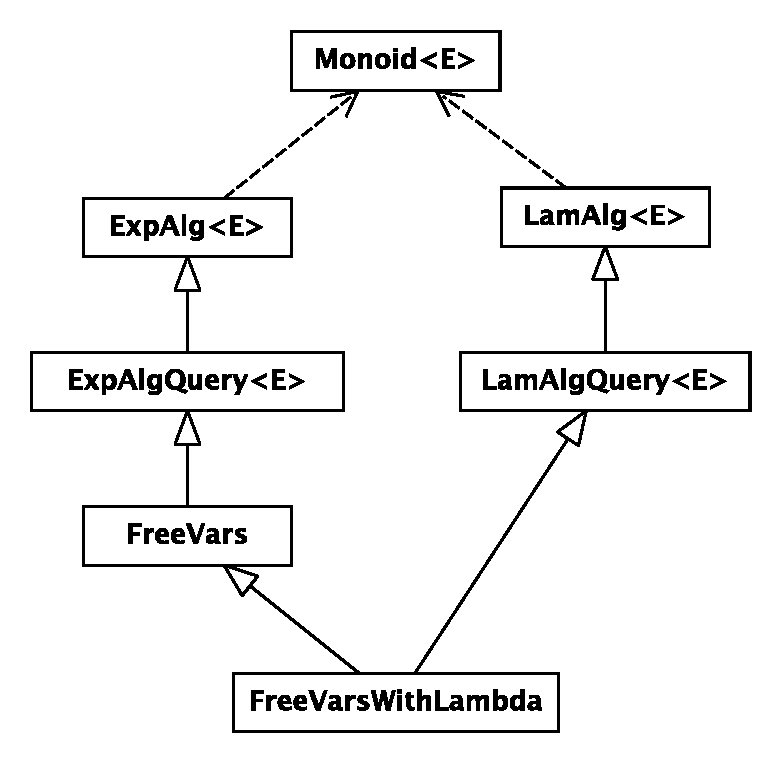
\includegraphics[width=0.45\linewidth]{extendQuery}
  \hspace*{2pt}
  \vline
  \hspace*{2pt}
  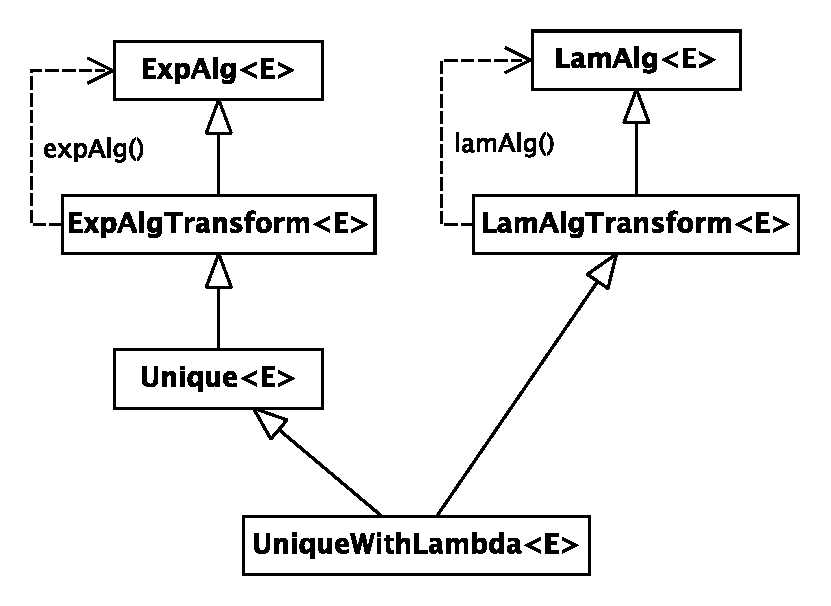
\includegraphics[width=0.45\linewidth]{extendTransform}
  
  \caption{Extension of the \texttt{FreeVars} query (left) and the \texttt{Unique} transformation}
  \label{FIG:extension}
\end{figure}

\noindent \name queries and transformation inherit  modular extensibility from the Object Algebra design pattern.
New transformations or queries are simply added by extending the interfaces generated by \name.
More interestingly, however, it is also possible to extend the data type with new constructors.
Here we briefly describe how queries and transformations can be extended in this case.
Figure~\ref{FIG:extension} gives a high level overview of the approach.


Consider the extension of the expression language with a lambda and application constructs.
In the Object Algebra style this is modeled as another interface, e.g., \lstinline{LamAlg}, which contains constructor methods to create lambdas (\lstinline{Lam}) and application expressions (\lstinline{App}).
The free variables query can then be extended as follows:

\lstinputlisting[linerange=18-22]{../ObjectAlgebras/src/expDemo3/FreeVarsWithLambda.java} % APPLY:linerange=EXTENDFREEVARS

This interface extends both the original \lstinline{FreeVars} query and the base query implementation that was generated for the \lstinline{LamAlg} interface defining the language extension.
Note again, that only the relevant method (\lstinline{Lam}) needs to be overridden. 


For transformations the pattern is similar.
To illustrate extension of transformation, consider the simple transformation that makes all variable occurrences unique.
This can be useful to distinguish multiple occurrences of the same name.

%% weird, computepositions does not compute the right range.
\lstinputlisting[linerange=4-7]{../ObjectAlgebras/src/expDemo3/Unique.java} % APPLY:linerange=UNIQUEVARS

This transformation uses a helper method \lstinline{nextInt()} which returns consecutive integers on each call.
The basic transformation simply renames \lstinline{Var} expressions.
If the expression language is extended with lambda constructs, the transformation needs to be extended as well.

\lstinputlisting[linerange=4-6]{../ObjectAlgebras/src/expDemo3/UniqueWithLambda.java} % APPLY:linerange=EXTEND_UNIQUEVARS

Note that the transformation uses the \lstinline{lamAlg()} algebra (generated in \lstinline{LamAlgTransfrom}),
to create lambda expressions.


%% Alternatively, a single method would suffice in the single-sorted case, since sub-classes or interfaces may refine the return type. 

%% \begin{lstlisting}[mathescape=true]
%% interface UniqueWithLambda<E, Alg extends ExpAlg<E> & LamAlg<E>>
%%     extends Unique<E>, LamAlgTransform<E> {	
%%   Alg expAlg();
  
%%   default E Lam(String x, E e) { return expAlg().Lam($...$); }
%% }
%% \end{lstlisting}




\section{Object Algebras Framework}

Generic queries, generalized generic queries, generic transformations and generalized generic transformations can help users write tree structure traversal code with more extensibility and flexibility. However, writing the generic query and transformation interfaces is still painful experience itself. It will be even better if the boilerplate code for tree structures can be generated automatically. If we pay more attention to our 4 query and transformation interfaces, without much difficulty we can find that the query and transform code structures for all \emph{Object Algebra Interfaces} share much similarity. Therefore we can make this code generation process automatic. 

To address this problem, we provide a framework \name, which utilizes \emph{Java Annotation} to generate query and transformation interfaces based on the \emph{Object Algebra Interface}. as illustrated below: 
\begin{lstlisting}[numbers=none] 
@Algebra
public interface ExpAlg<Exp> {
	Exp Var(String s);
	Exp Lit(int i);
	Exp Add(Exp e1, Exp e2);
}
\end{lstlisting}

With the annotation "$@$Algebra", the framework will generate the boilerplate codes for us automatically. As for our ExpAlg example, the following directory structure will be generated by the library. 
\dirtree{%
 .1 src/.
 .2 query/.
 .3 ExpAlgQuery.
 .3 G\_ExpAlgQuery.
 .2 transform/.
 .3 ExpAlgTransform.
 .3 G\_ExpAlgTransform.
}

Here the automatically generated ExpAlgQuery, G\_ExpAlgQuery, ExpAlgTransform and G\_ExpAlgTransform are exactly the same code as we discussed in the previous sections. Furthermore, the monoid interface is also included in the \emph{Object Algebra Framework}.

Hence when programming with query and transformations, the programmer can skip the intermediate steps such as constructing generic queries and transformations, but only focus on rewriting the interesting cases. For instance, in our ExpAlg example, to implement FreeVars algebra, we can simply override the \lstinline{Exp Var(String s)} method of \lstinline{class ExpAlgQuery} to return variable name, and provide the specific monoid needed, which in this case will be a \lstinline{StringListMonoid}. While the SubstVars algebra can be realized by overriding the \lstinline{Exp Var(String s)} method of ExpAlgTransform interface, which substitutes variable names as specified. 


\section{Case Study}

To illustrate the utility of \name we have implemented a number of queries and transformations in the context of QL, a simple DSL for questionnaires implemented using Object Algebras~\cite{gouseti14extensible}.
A questionnaire is rendered as an interactive form where, depending on user actions, new questions may appear, or values may be computed.
An example QL questionnaire is shown on the left of Fig.~\ref{FIG:houseowning} together with its rendering on the right.

QL programs consist of lists of labeled, typed questions.
Questions can be answerable, meaning the user has to enter some data, or computed, in which case the question is defined by an expression.
A conditional if-then-else construct allows questions to visually appear only when a certain condition is true.

\begin{figure}[t]
\hspace*{-5pt}\begin{minipage}{0.6\linewidth}
\begin{lstlisting}[language=ql]
form HouseOwning {
  soldHouse: "Did you sell a house?" boolean
  boughtHouse: "Did you buy a house?" boolean
  if (soldHouse) {
    sellingPrice: "Selling price:" integer
    privateDebt: "Private debts:" integer
    valueResidue: "Value residue:" integer 
       = (sellingPrice - privateDebt)
  }
}
\end{lstlisting}
\end{minipage}
\begin{minipage}{0.5\linewidth}
  \includegraphics[width=\linewidth]{sections/screenshot}
\end{minipage}
\caption{Example QL questionnaire (left) and its rendering (right)}
\label{FIG:houseowning}
\end{figure}

\subsection{QL queries and transformation}

The queries extract derived information from a QL program, such as the set of used variables, the data and control dependencies between questions and the global type environment.
The transformations include two transformations of language extensions to the base language.
The first realizes a simple desugaring of ``unless(c){...}'' to ``if(not(c)){...}''.
The second desugaring statically unfolds a constant bound loop construct (``repeat (i){...}'') and renames variables occurring below it accordingly.
Finally, we have implemented a simple rename variable operation, and a normalizer which inlines the conditions of nested if-then constructs.  

Table~\ref{TBL:qlresults} shows the number of cases that had to be overridden to implement each particular operation. The second column shows the number of  constructs for each sort in QL (Form, Stmt, and Exp).
As can be seen, none of the operations required implementing all cases.
The bottom row shows the number of overridden cases as a percentage.
For this set of queries and transformations, almost no expression cases needed to be overridden, except the ``Var'' case in collect variables, rename variable and desugar ``repeat''\footnote{Note, however, that the dependency extraction queries reuse the collect variables query on expressions.}.
The cases required for desugaring include the case of the language extension (e.g. \lstinline{Unless} and \lstinline{Repeat}, respectively). These cases are not counted in the total in the second column but are used to compute the percentage. 

%% \begin{table}[t]
%%   \centering
%%   \begin{tabular}{l|c|c|c}
%%     Operation            & Exp (18) & Stmt (5) & Form (1) \\\hline
%%     Collect variables    & 1        &          &          \\
%%     Data dependencies    &          & 3        & 1        \\
%%     Control dependencies &          & 4        & 1        \\
%%     Type environment     &          & 2        &          \\\hline
%%     Rename variable      & 1        & 2        &          \\
%%     Inline conditions    &          & 4        &          \\
%%     Desugar ``unless''   &          & 1        &          \\
%%     Desugar ``repeat''   & 1        & 3        &          \\
%%   \end{tabular}
%%   \caption{Number of overriden cases per query and transformation in
%%     the context of the QL implementation\label{TBL:qlresults}}
%% \end{table}

\def\rot#1{\rotatebox{90}{#1}}

\begin{table}[t]
  \centering
  \begin{tabular}{lccccccccc}
    Sort & \rot{\#Cases} & \rot{Collect vars} & \rot{Data deps} & \rot{Control deps} & \rot{Type env} & \rot{Rename var} & \rot{Inline conds} & \rot{\texttt{unless}} & \rot{\texttt{repeat}} \\\hline
    Form & 1             &                    & 1               & 1                  &                &                  &                    &                       &                       \\
    Stmt & 5             &                    & 3               & 4                  & 2              & 2                & 4                  & 1                     & 3                     \\ 
    Exp  & 18            & 1                  &                 &                    &                & 1                &                    &                       & 1                     \\\hline
         &               & 4\%                & 17\%            & 21\%               & 8\%            & 13\%             & 17\%               & 4\%                   & 16\%                  \\
  \end{tabular}
  \vspace*{.1in}
  \caption{Number of overriden cases per query and transformation in
    the context of the QL implementation\label{TBL:qlresults}}
\end{table}


%% \subsection{Extending queries and transformations}

%% Instead of desugaring language extensions to the base language it is also possible to treat them as first-class constructs and retroactively extend existing queries and transformations.
%% The framework permits to use  Java interface extension to achieve this in a fully type safe way.
%% Figure~\ref{inline_conds_unless} and Fig.~\ref{controldeps_unless} show the extension of the inline conditions transformation and control dependencies query when extending QL with ``unless''.

%% \begin{figure}[tb]
%% \lstinputlisting[linerange=9-14]{../QL/src/_syb/trafo/InlineConditionsUnless.java} % APPLY:linerange=INLINECONDS_UNLESS
%% \vspace{-.1in}
%% \caption{Extending the inline-conditions transformation to deal with ``unless''}
%% \label{inline_conds_unless}
%% \end{figure}

%% \begin{figure}[tb]
%% \lstinputlisting[linerange=10-18]{../QL/src/_syb/query/ControlDepGraphUnless.java} % APPLY:linerange=CONTROLDEPS_UNLESS
%% \vspace{-.1in}
%% \caption{Extending the control-dependencies query to deal with ``unless''}
%% \label{controldeps_unless}
%% \end{figure}

%% Inlining of conditions across ``unless'' statements (Fig.~\ref{inline_conds_unless}) is analogous to the implementation for ``if''.
%% It involves creating a conjunction of the input (\lstinline{guard}) and the negated condition and then passing it down the body of ``unless''. The result is the inlined version of the body.
%% The extension of the control dependencies (Fig.~\ref{controldeps_unless}) query simply delegates to the implementation of ``if'' (\lstinline{iff}). 

\subsection{Chaining transformations}

A typical compiler consists of many transformations chained together in a pipeline.
\name transformations support this pattern by passing transformation algebras as the base algebra to the implementation of another transformation.
For instance, the desugar unless transformation desugars the ``unless'' statement to ``if'' statements in another algebra.
The latter can represent yet another transformation.

In the context of QL, ``unless'' desugaring, condition inlinging and variable renaming can be chained together as follows:

  \lstinputlisting[linerange=162-162]{../QL/src/_syb/trafo/TestPipelining.java} % APPLY:linerange=PIPELINEQL

The chained transformation \lstinline{alg} first desugars ``unless'', then inlines conditions, and finally renames variables according to the map \lstinline{ren}.
The \lstinline{Rename} transformation gets as base algebra an instance of \lstinline{Format}, a pretty printer for QL. 

The algebra \lstinline{alg} can now be used to create questionnaires:

  \lstinputlisting[linerange=166-168]{../QL/src/_syb/trafo/TestPipelining.java} % APPLY:linerange=PIPELINEQL_CALL

The result of constructing this simple questionnaire is a function object representing the ``to be inlined'' representation of the questionnaire after desugaring.
The \lstinline{IFormatWithPrecedence} and \lstinline{IFormat} types are  formatting operations, respectively representing expressions and statements; these types originate from the \lstinline{Format} algebra passed to \lstinline{Rename}.
Calling this function with a boolean expression representing \lstinline{true} will trigger inlining of conditions and renaming. The result is then a formatting object (\lstinline{IFormat}) which can be used to print out the transformed questionnaire:

  \begin{lstlisting}[language=ql]
    form myForm {
      if (true && !y) y "X?" boolean
    }
  \end{lstlisting}

  As can be seen, the variable \lstinline{x} has been renamed to \lstinline{y}.
The (renamed) condition \lstinline{y} is now negated, because of the desugaring of ``unless''.
Finally, the result of inlining conditions can be observed from the conjunction in the \lstinline[language=ql]{if} statement.

  
\subsection{\name performance vs Vanilla ASTs}

\begin{figure}[t]
  \hspace*{-.1\textwidth}
  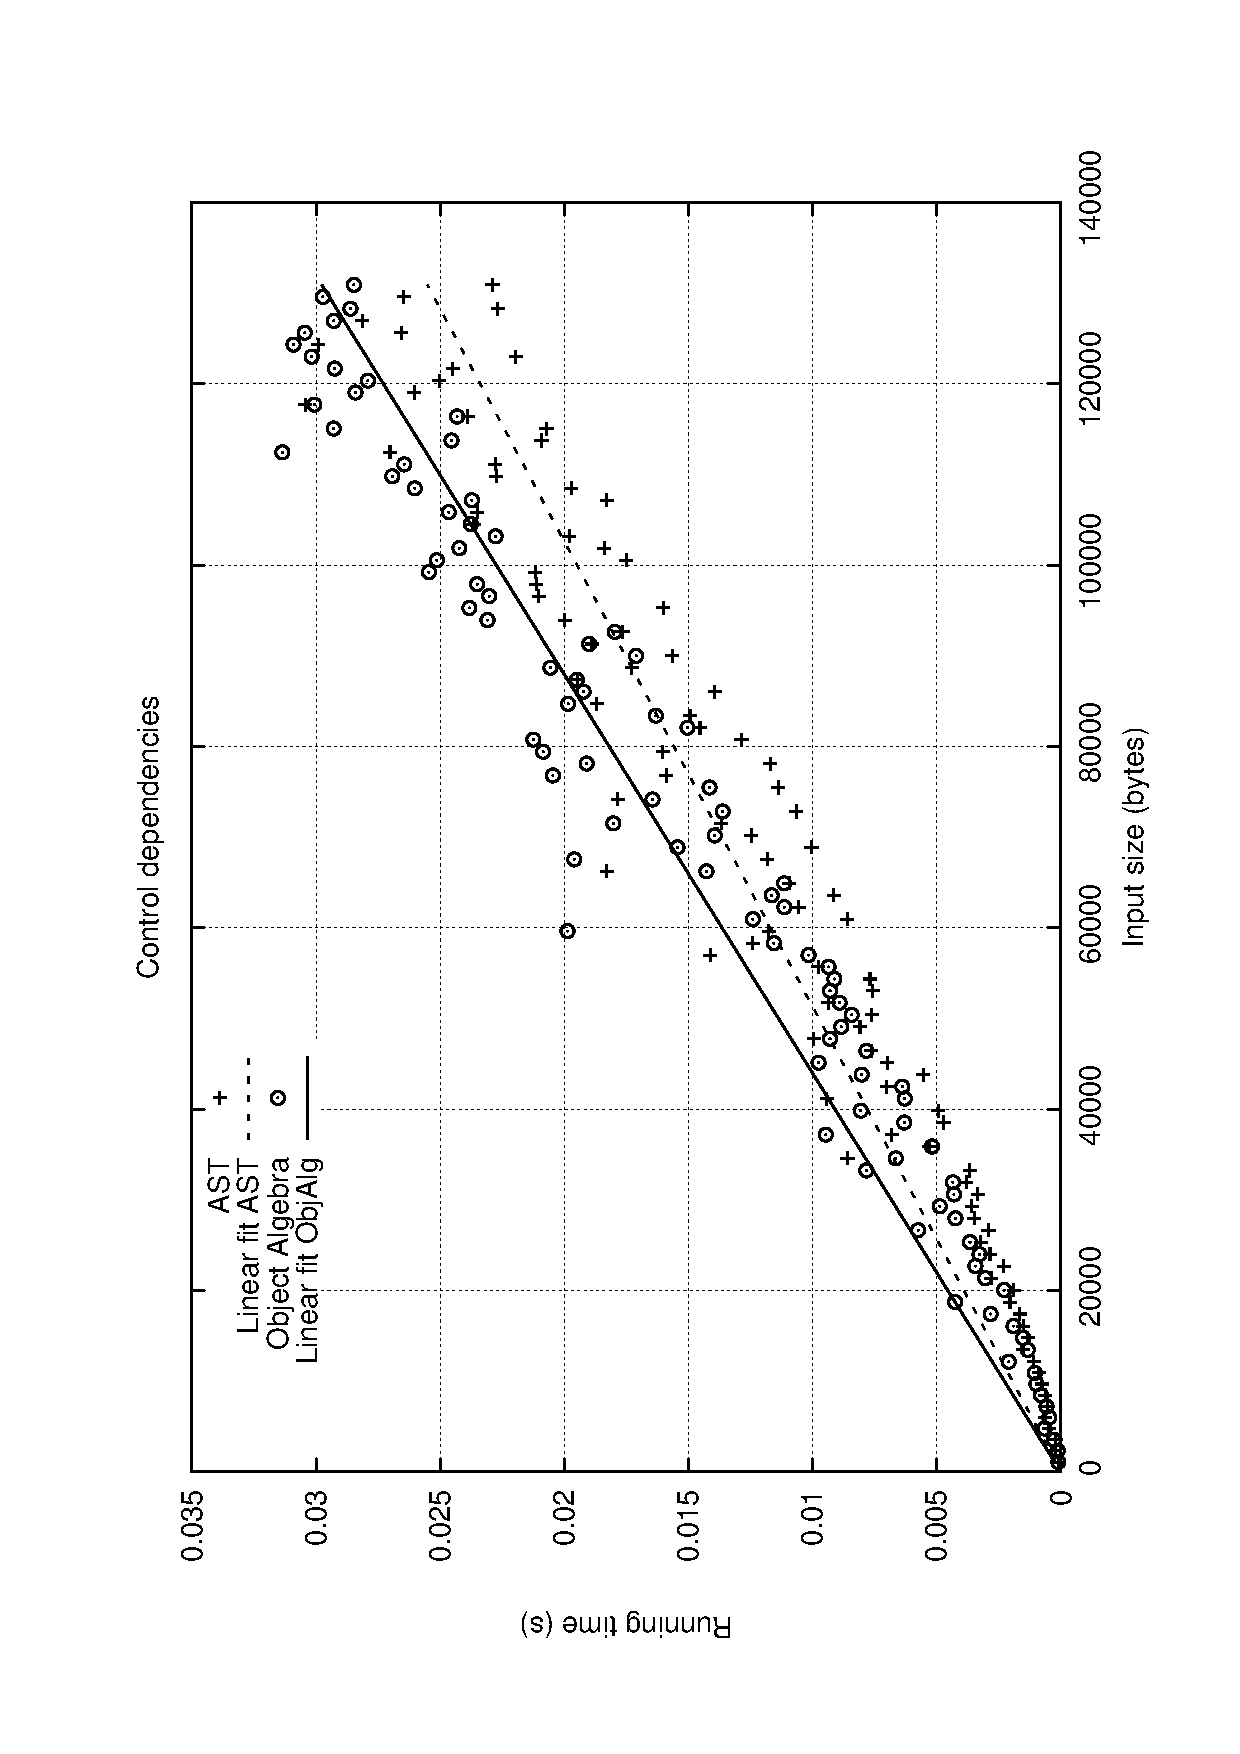
\includegraphics[width=0.56\textwidth]{plots/controldeps}
  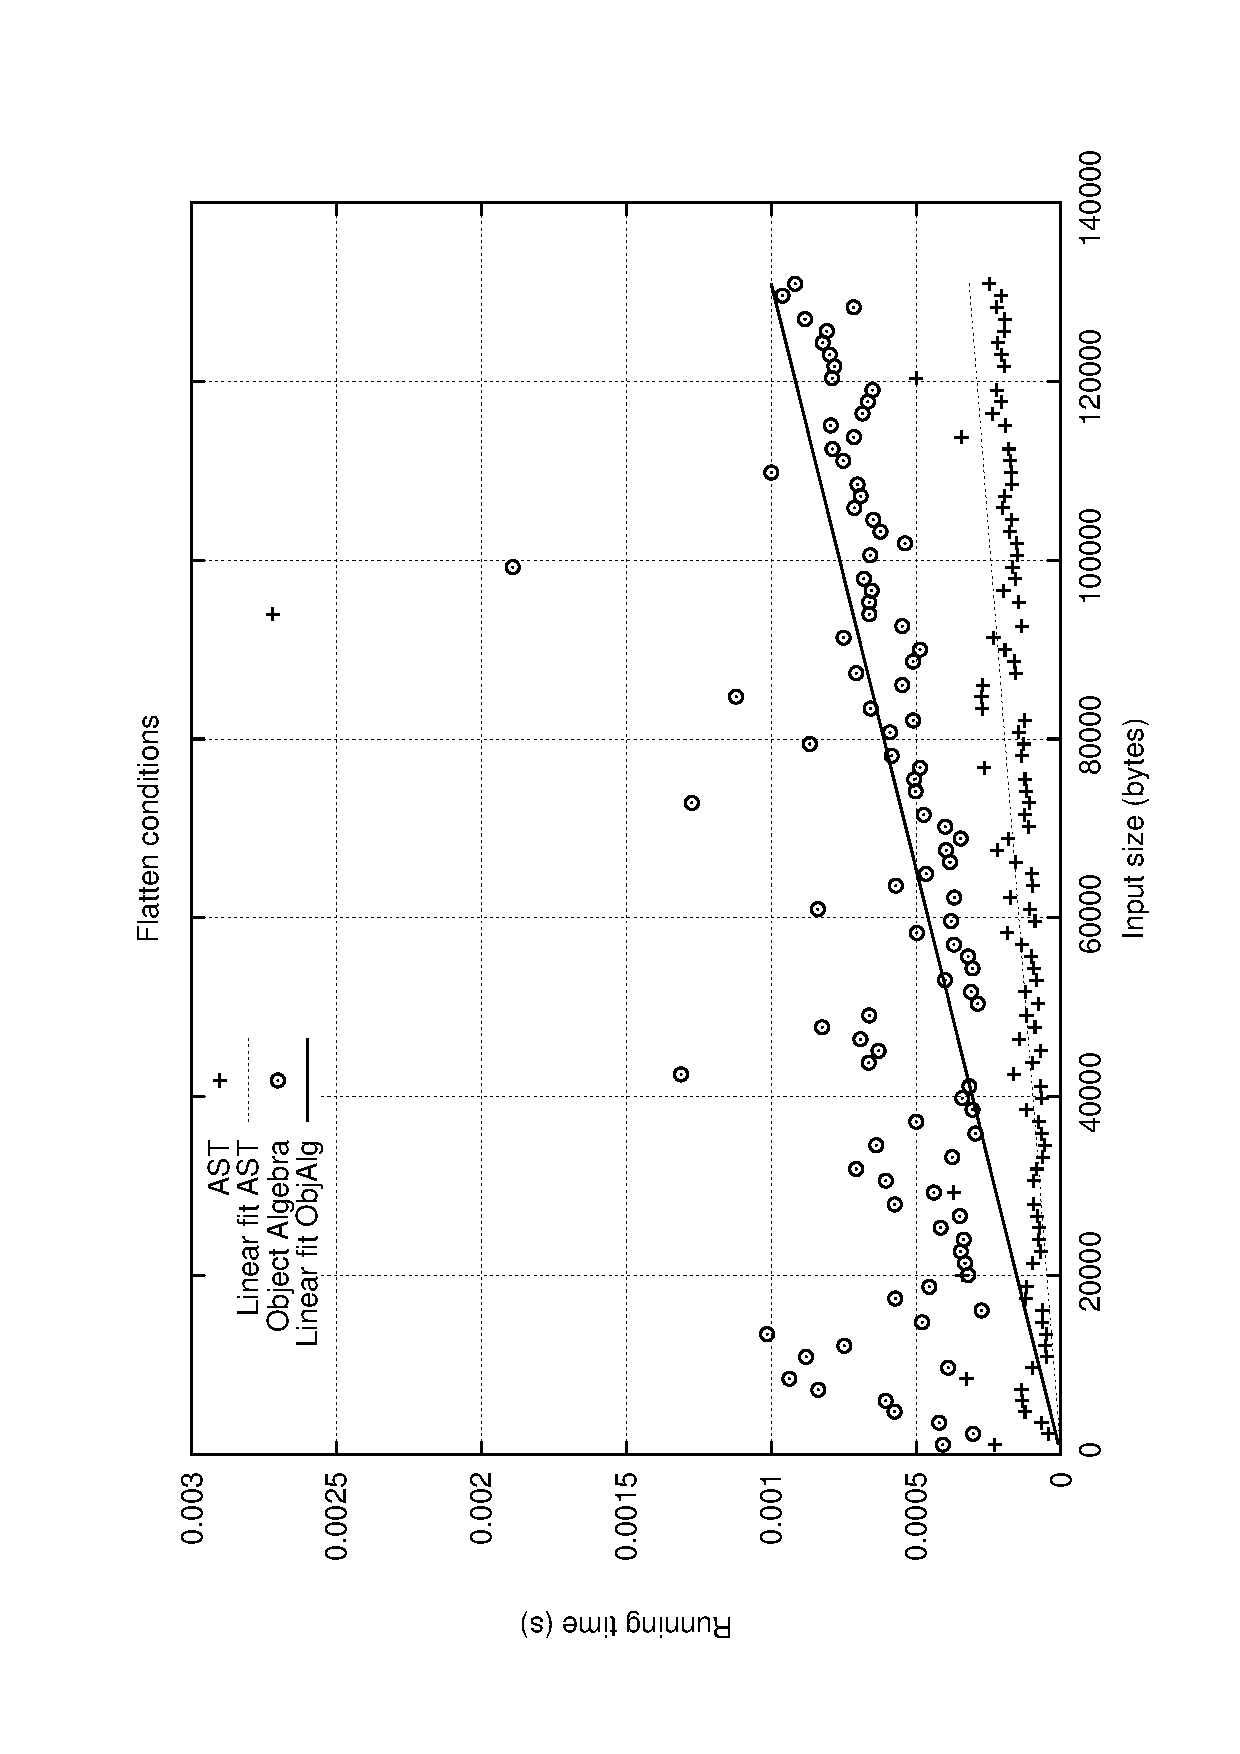
\includegraphics[width=0.56\textwidth]{plots/inline}
  \caption{Performance comparison of control dependencies query (left) and inline conditions transformation (right) implemented using normal ASTs vs using the \name framework\label{FIG:performance}}
\end{figure}

We compared the performance characteristics of the operations implemented using \name with respect to vanilla implementations based on ordinary AST classes with ordinary methods representing the transformations and queries.
The operations were executed on progressively larger QL programs (up to 140Kb).
In the vanilla implementation, the program was parsed into an AST structure, and then the operation was invoked and measured.
In the case of the \name queries, constructing the ``AST'' corresponds to executing the query, so we measured that.
For context-dependent transformations, however, building the ``AST'' corresponds to constructing the function to execute the transformation, hence we only measured the execution of invoking this function. 
To make the comparison as fair as possible, the vanilla query implementations use the same monoid structures as in \name.

The comparison of the control dependencies query is shown on the left of Fig.~\ref{FIG:performance}.
The plot shows that the performance is quite comparable.
On average, the \name implementation of the query seems a little slower.
This is probably caused by the extensive use of interfaces in the \name framework, whereas the AST-based implementation only uses abstract and concrete classes
%\tijs{NEED REFERENCE!!!!, but see: \url{http://stackoverflow.com/questions/6839943/why-are-interface-method-invocations-slower-than-concrete-invocations}}.
For transformations the performance difference is slightly more pronounced.
The right of Fig.~\ref{FIG:performance} shows the performance comparison of the inline conditions transformation. 
The greater difference can be explained by the fact that creating a new structure in a \name transformation involves dynamically dispatched method calls instead of statically bound constructor calls. 






\section{Related Work}\label{sec:related}

To the best of our knowledge, few work has been done addressing writing generic queries and transformations with object algebras, while we should mention some work on object algebras and large tree structures traversal control, which inspired and formed the basis of our work. 

\textit{Object Algebras}. Oliveira proposed Object Algebras as a solution to Expression Problem. Object algebras applies well in mainstream object oriented languages like Java. It is a lightweight solution in terms of language features required. Oliveira also worked on using intersection type and type-constructor polymorphism to make object algebras compositional with feature oriented programming. Different from their prior research, we found that when applying object algebras in rich tree structures, boilerplate code is hard to avoid. Hence our work focuses on reducing the amount of boilerplate code for developers when writing queries and transformations with object algebra tree structures. 

\textit{Tree structures traversals}. In the functional programming community like Haskell, much research has been done on traversal control of large structures. Lammel's Scrap your Boilerplate\cite{ralf03syb} series introduced a practical design pattern for generic programming in tree structures, which inspired our work of scrapping boilerplates in Object Algebras. Bringert\cite{bjorn08acf} introduced useful compositional functions to help construct final results in Haskell. Lammel\cite{ralf00banana} proposed a polytypic programming approach for generalized and basic folds. These fold algebras scale up applications involving large systems of mutually recursive datatypes. These works all try to optimize traversal control of large structures in functional programming paradigm, while our work solves a similar problem in Object Algebras, a programming style in Object Oriented Programming paradigm. 

\textit{Visitor Combinators and Traversal Control}. Visser\cite{visser01visitor} provided some visitor combinators that can express interesting traversal strategies in visitor pattern. We applies some similar idea like identity transformation in simple transformation, but our work targets at traversal control in Object Algebras. 

In summary, prior to our work, research has been done on object algebras and composition problem of this programming style. In the functional programming world and with visitor pattern, traversal control in large structures is also explored. Different from these work, we explored techniques helping write generic queries and transformations traversing large tree structures with Object Algebras. 



\section{Conclusion}\label{sec:conclusion}

This paper showed how various types of traversals for complex
structures can be automatically provided by \Name. \name traversals are
written directly in Java and are type-safe, extensible and separately
compilable. There has always been a tension between the 
correctness guarantees of static typing, and the flexibility of
untyped/dynamically-typed approaches. \name shows that even
in type systems like Java's, it is possible to get considerable
flexibility and adaptability for the problem of boilerplate code in
traversals of complex structures, without giving up modular static typing. 
%\name offers the best of both worlds: the
%static typing guarantees; and flexibility and adaptability.

There are many of avenues for future work. One area of research is to
extend \name traversals to support flexible traversal strategies,
similarly to strategic
programming~\cite{borovansky1996elan,visser1998core,vandenBrand:2003:TRT:941566.941568}. Another
line of work worth exploring is to adopt generalizations of object
algebras~\cite{oliveira13fop} for added expressiveness of \name
traversals.




\bibliographystyle{splncs}
\bibliography{paper}

\appendix

\end{document}
